\begin{enumerate}[label=\thesection.\arabic*.,ref=\thesection.\theenumi]
\numberwithin{equation}{enumi}


\item  Sketch the polar plot for the transfer function
\begin{align}
\label{ee18btech11051_eq1}
     G(s) = \frac{10(s+1)}{10+s}
\end{align} for \\0 $\leq \omega < \infty$.
Which quadrant does it lie in?
\\
\solution Substituting s = $\j \omega$ in \eqref{ee18btech11051_eq1},
\begin{align}
\label{ee18btech11051_eq2}
G\brak{\j\omega} &= \frac{10(1+\j\omega)}{(10+\j\omega)}\\
 \label{ee18btech11051_eq3}
&= \underbrace{10\sqrt{\frac{1+\omega^2}{100+\omega^2}}}_{r}
\nonumber \\
&\quad \times \exp\cbrak{\j\underbrace{\brak{\tan^{-1}(\omega)-\tan^{-1}\brak{\frac{\omega}{10}}}}_{\theta}}
\end{align}
%
\begin{align}
\because \frac{d}{d\omega}\tan^{-1}(\omega) = \frac{1}{1+\omega^2}, \omega > 0,
\end{align}
%
$\tan^{-1}(\omega) $ is an increasing funtion.  Hence, 

\begin{align}
\tan^{-1}(\omega) \geq \tan^{-1}\brak{\frac{\omega}{10}}.
\end{align}
$\because $ $0 < \theta < \frac{\pi}{2}$ in \eqref{ee18btech11051_eq3}, the polar plot of $G(s)$ lies in the first quadrant. The following code generates the polar plot in Fig.       \ref{fig:ee18btech11051_fig2}.
%
\begin{lstlisting}
    codes/ee18btech11051.py
\end{lstlisting}

      \begin{figure}[!h]
      \centering
      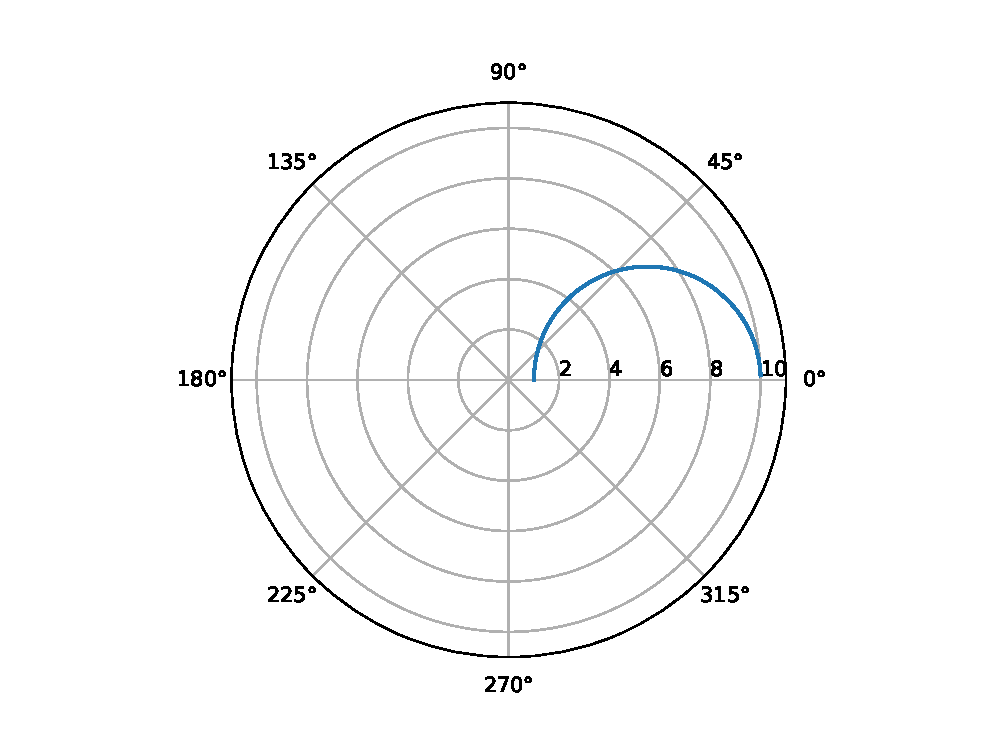
\includegraphics[width=\columnwidth]{./figs/ee18btech11051.eps}
      \caption{}
      \label{fig:ee18btech11051_fig2}
      \end{figure}



\end{enumerate}
